
\chapter{Curves of genus 4 and 5}\label{genus 4, 5 Chapter}

In this chapter we
study
the linear series that exist on curves of genus 4 and 5, and what this says
about maps to $\PP^r` `$, focusing as usual on the nonhyperelliptic case.

\section{Curves of genus 4}

In genus 4 we
face
\index{genus 4 curve|(}%
a question that the elementary theory based on the Riemann--Roch
formula cannot answer: are nonhyperelliptic curves of genus 4
\index{trigonal}%
\index{cover!3-sheeted}%
\emph{trigonal}, that is, expressible as 3-sheeted covers of $\PP^1$?
The answer will emerge from our analysis in
Proposition~\ref{genus 4 trigonal}.

\subsection*{The canonical model}

Let $C$ be a nonhyperelliptic curve of genus 4. The canonical map $\phi_K : C \hookrightarrow \PP^3$  embeds $C$ as a curve of degree 6 in $\PP^3` `$, and we identify $C$ with the image.  As in previous cases we may describe the homogeneous ideal  $I$ of $C$ by considering the restriction maps
\index{canonical curve!of genus 4}%
$$
\rho_m : H^0(\cO_{\PP^3}(m)) \; \to \; H^0(\cO_{C}(m)) = H^0(mK_C).
$$
If
$m=2$ we have $\h^0(\cO_{\PP^3}(2)) = \tbinom{5}{3} = 10$, while by the
\index{Riemann--Roch theorem}%
Riemann--Roch theorem
$$
h^0(\cO_C(2)) = 12 - 4 + 1 = 9.
$$
Thus $C \subset \PP^3$  lies on at least one quadric surface $Q$. The quadric $Q$ must be irreducible, since any reducible and/or nonreduced quadric must be a union of planes, and thus cannot contain an irreducible nondegenerate curve.
If $Q'\subset\nobreak \PP^3$ is another quadric then, by B\'ezout's theorem,
$Q\cap Q'$ is a curve of degree 4 and thus
cannot
contain $C$. From
this we see that $Q$ is unique, and it follows that $\rho_2$ is surjective.

What about cubics? Again we consider the restriction map
$$
\rho_3 : H^0(\cO_{\PP^3}(3)) \; \to \; H^0(\cO_{C}(3)) = H^0(3K_C).
$$
The space $H^0(\cO_{\PP^3}(3))$ has dimension $\tbinom{6}{3} = 20$, while  the Riemann--Roch formula shows that
$$
h^0(\cO_C(3)) = 18 - 4 + 1 = 15.
$$
It follows that the ideal of $C$ contains at least a 5-dimensional vector space of cubic polynomials. We can get a 4-dimensional subspace as products of the unique quadratic polynomial $F$ vanishing on $C$ with linear forms\emdash these define the cubic surfaces containing $Q$. Since $5 > 4$ we  conclude that the curve $C$ lies on at least one cubic surface $S$  not containing $Q$.
B\'ezout's theorem
\index{Bezout@B\'ezout's theorem}%
shows that the curve $Q \cap S$ has degree 6; thus it must be equal to $C$.

Let $G=0$ be the cubic form defining the surface $S$. By
Lasker's theorem
\index{Lasker's theorem}%
the ideal $(F,G)$ is unmixed,
and thus is equal to the homogeneous ideal of $C$.

Conversely,
let $C = Q\cap S$ with $Q$ a quadric and $S$ a cubic. By Corollary~\ref{canonical of complete intersection} the canonical sheaf of $C$ is
$$
\omega_C = (\omega_{Q} \otimes \cO_{Q}(3))|_C = \cO_C(-2+3) = \cO_C(1)
,
$$
so $C$ is a canonical curve. Since $C$ is smooth, the quadric and the cubic must meet transversely at points that are nonsingular on each of them. Thus:

\begin{theorem}
\label{canonical genus 4}
The canonical model of a nonhyperelliptic curve of genus $4$ is a
\index{complete intersection!of quadric and cubic in $\PP^3$}%
\index{P@$\PP^3$}%
complete intersection of a quadric $Q = V(F)$ and a cubic surface
$S=V(G)$ meeting transversely along nonsingular points of each.
Conversely, any smooth curve that is the complete intersection of a
quadric and a cubic surface in $\PP^3$ is the canonical model of a
nonhyperelliptic curve of genus $4$.\qed
\end{theorem}

Since the quadric surface $Q$ containing the canonical curve $C$
is unique, its rank is an invariant of $C$.
Since $C$ is irreducible and nondegenerate, the quadric cannot be a
double plane or the union of two planes, but it can be singular
(rank~3) or smooth (rank 4). On the other hand, the singularities of a
cubic~$S$ such that $S\cap Q = C$ play no role. Of course $S$ must be
nonsingular along~$C$, since else
$C$ would be singular. We can vary $S$ by adding a multiple of the
equation of $Q$ to the equation of $S$, and since this linear series
of cubics has base locus only along $C$,
Bertini's theorem
\index{Bertini's theorem}%
shows that the general such cubic is nonsingular everywhere.

\subsection*{Maps to projective space}

\subsubsection*{Maps to $\PP^1$}

We can now answer the question we asked at the outset, whether a
nonhyperelliptic curve of genus 4 can be expressed as a 3-sheeted
\index{cover!3-sheeted}%
cover of $\PP^1` `$. This amounts to asking if there are any divisors
$D$ on $C$ of degree 3 with $r(D) \geq 1$; since we can take $D$ to be
a general fiber of a map $\pi : C \to \PP^1` `$, we can for simplicity
assume $D = p+q+r$ is the sum of three distinct points.

By the
geometric Riemann--Roch theorem,
\index{Riemann--Roch theorem!geometric}%
a divisor $D = p+q+r$ on a canonical curve $C \subset \PP^{g-1}$ has
$r(D) \geq 1$ if and only~if the three points $p,q,r \in C$ are
collinear. If three points $p,q,r \in C \subset Q$ lie on a line $L
\subset \PP^3$ then the quadric $Q$ will meet $L$ in at least three
points, and hence will contain $L$. Conversely,  if $L$ is a line
contained in $Q$, then the divisor $D = C \cap L = S \cap L$ on $C$
has degree  3. Thus we can answer our question in terms of the family
of lines contained in $Q$.

Any smooth quadric is isomorphic to $\PP^1\times \PP^1` `$, and
contains two families of lines, or
\index{ruling}%
\emph{rulings}.
On the other hand,
any  quadric of rank 3 is a
cone
\index{cone!quadratic}%
over a smooth plane conic, and thus
has just one ruling. By the argument above, the pencils of divisors on
$C$ cut out by the lines of these rulings are the $g^1_3$s on $C$.
This proves:

\begin{proposition}\label{genus 4 trigonal}
A nonhyperelliptic curve of genus $4$ may be expressed as a
$3$-sheeted cover of $\PP^1$ in either one or two ways, depending on
whether the unique quadric containing the canonical model of the curve
is singular or smooth.
\unif
\end{proposition}

See Figure~\ref{Fig8.1} for an idea how this might look in
each case.

\begin{figure}
\centerline{\raise3pt\hbox{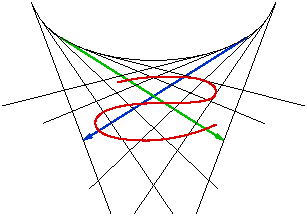
\includegraphics[height=1.93in]{main/Fig08-1}}\hfil
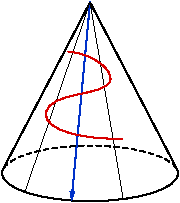
\includegraphics[height=2in]{main/Fig08-2}\quad}
\caption{Left: canonical curve of genus 4 on a smooth quadric, showing
  two $g^{1}_3$s.  Right: canonical curve of genus 4 on a quadric
  cone, with just one~$g^{1}_{3}$.}
\label{Fig8.1}
\end{figure}

Putting together
the analyses of the preceding sections, we have shown that
\index{hyperelliptic-trigonal dichotomy for curves of genus $\leq 4$}%
\emph{every curve of genus $g$ with $2\leq g \leq 4$ is either hyperelliptic or trigonal}.

\subsubsection*{Maps to $\PP^2$}

We can also describe the lowest degree plane models of nonhyperelliptic curves $C$ of genus 4.
We can get a plane model of degree 5 by projecting $C$ from a point $p$ of the canonical model of $C$.
Moreover, the
Riemann--Roch theorem
\index{Riemann--Roch theorem}%
shows that if $D$ is a divisor of
degree 5 with $r(D)=2$ then
$\h^0(K-D) = 1$. Thus $D$ is of the form
$K-p$ for some point $p \in C$, and the map to $\PP^2$ corresponding
to $D$ is $\pi_p$. These  maps $\pi_p: C\to \PP^2$ have the lowest
possible degree (except for those whose image is  contained in a line)
because by
Clifford's theorem
\index{Clifford's theorem}%
a nonhyperelliptic curve of genus 4
cannot have a $g^2_4$.

We now consider the singularities of the
plane quintic
\index{plane quintic}%
$\pi_p(C)$.
Suppose as above that $C = Q\cap S$, with $Q$ a quadric. If a line $L$
through $p$ meets $C$ in $p$ plus a divisor of degree $\geq 2$ then,
as we have seen, $L$ must lie in $Q$.  Any line through $p$ that is
not contained in $Q$ meets $C$ in at most a single reduced point,
whose image is thus a nonsingular point of $\pi(C)$. Moreover, a line
that met $C$ in a divisor of degree 4 or more
would have to lie in both the quadric and
the cubic containing $C$, and therefore would be contained in $C$.
Since $C$ is irreducible there can be no such line; thus the image
$\pi_p(C)$ has at most double points.

We distinguish two cases, depending on whether
the quadric $Q$ is smooth or singular. We will make use of the
Gauss map
\index{Gauss map}%
of the quadric,
described by the next lemma.

\begin{lemma}
Let $L \subset S \subset \PP^3$ be a line on a surface $S \subset \PP^3$ of degree $d \geq 2$, and
write $S_{\sing}$ for the singular locus of $S$. The Gauss map $\cG :
S \to (\PP^3)^*$ sending each point $p \in S\setminus S_{\sing}$ to
the tangent plane $\TT_p(S)$ maps $L$ into the
dual line
\index{dual line|defi}%
\index{duality}%
in $\PP^3$ (that is, the locus of planes containing $L$); if $S$ is
smooth along $L$ then $\cG$  has degree $d-1$, and if $S$ is singular
anywhere along $L$ it has strictly lower degree.
\unif
\end{lemma}

The geometric idea behind this result is easy to understand: If $S$ is
smooth along $L$ and $H\cong \PP^{2}$ is a plane containing $L$, then
$H\cap S = L \cup D$ for a plane curve $D$ of degree $d-1$. The plane
$H$ is tangent to $S$ at a point $p$ if and only~if $H\cap S$ is
singular at $p$; and this occurs at each of the $d-1$ points (counted
with multiplicity) at which $D$ meets $L$, suggesting that the
restriction of the Gauss map is $(d{-}1)$-to-one in this case.

If $S$ is singular somewhere along $L$, then every plane through that point would be among the tangent
planes in the sense above, and the image of $L$ would be a component of a curve of degree $d-1$ containing a line; thus of lower degree.

To see that the multiplicities count correctly in this argument, we will give an algebraic version:
\unif

\begin{proof}
Suppose that in terms of homogeneous coordinates $[X,Y,Z,W]$ on $\PP^3$ the line $L$ is given by $X = Y = 0$. Then the defining equation $F$ of $S$ can be written
$$
F(X,Y,Z,W) = X\cdot G(Z,W) + Y\cdot H(Z,W) + J(X,Y,Z,W)
$$
where $J$ vanishes to order 2 along $L$; that is, $J \in (X,Y)^2` `$. The Gauss map $\cG|_L$ restricted to $L$ is then given by
$$
[0,0,Z,W] \mapsto [G(Z,W), H(Z,W), 0, 0].
$$
The polynomials $G$ and $H$ have degree $d-1$, and have a common zero if and only~if $S$ is singular somewhere along $L$; the lemma follows.
\end{proof}

\begin{example}[Gauss map of a quadric]
\label{Gauss of Quadric}
Let $Q\subset \PP^3$ be a smooth quadric,
\index{Gauss map!of a quadric}%
\index{quadric surface!Gauss map}%
and let $L\subset Q$ be the line $X=Y =0$. Since we may write the
equation of $Q$ as $XZ+YW = 0$, the Gauss map of $Q$, restricted to
$L$, maps $L$ one-to-one onto the dual line. Indeed, the
Gauss map
takes $Q$ isomorphically onto its dual, which is also a smooth quadric.

 We can also see this geometrically: if $H \subset \PP^3$ is any plane containing the line $L \subset Q$, then $H$ intersects $Q$ in the union of $L$ and a line $M$; the hyperplane section $Q \cap H = L \cup M$ is then singular at a unique point $p \in L$. Thus the Gauss map gives a bijection between points on $L$ and planes containing $L$.
\unif
\end{example}

Given this, we can analyze the geometry of projections $\pi_p(C)$ of our canonical curve $C = Q \cap S$ as follows:

\begin{enumerate}
\item $Q$ is nonsingular:
In this case there are two lines $L_1, L_2$ on $Q$ that pass through
$p$; they meet $C$ in $p$ plus divisors $E_1$ and $E_2$ of degree 2.
If each $E_i$ consists of distinct points then, since the tangent
planes to the quadric along $L_i$ are all distinct by
Example~\ref{Gauss of Quadric}, the plane curve $\pi(C)$ has two
nodes, one at the image of each $E_i$.

On the other hand, if $E_i$ consists of a double point $2q$ (that is,
$L_i$ is tangent to $C$ at $q\neq p$, or meets $C$ three times at
$q=p$), then $\pi(C)$ has a cusp at the corresponding image point.

In either case, $\pi(C)$ has two distinct singular points, each either a
node or a cusp. The two $g^1_3$s on $C$ correspond to the
projections from these singular points. These possibilities are
illustrated in Figure~\ref{Fig8.2A}.

\begin{figure}[b]
\centerline {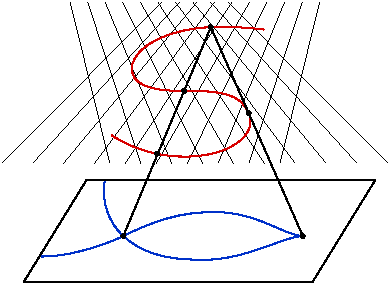
\includegraphics[height=2in]{main/canonical-projected-2}}
\caption{If a genus 4 canonical curve $C$ lies on a smooth quadric, the image of the projection of $C$ from a point $p\in C$
is a
plane quintic
\index{quintic curve}%
\index{canonical curve!of genus 4}%
with two singular points.
\hbox to 50pt{} % avoid extra jump before short line
}
\label{Fig8.2A}
\end{figure}

\item $Q$ is a
cone:
\index{cone!quadratic}%
In this case, since the curve cannot pass through the singular point
of $Q$ there is a unique line $L\subset Q$ that passes through $p$.
Let $p+E$ be the divisor on $C$ in which this line meets $C$. The
tangent planes to $Q$ along $L$ are all the same. Thus if
$E = q_1+q_2$ consists of two distinct points,
the image $\pi_p(C)$ has two smooth branches sharing a common tangent line at
$\pi_p(q_1) = \pi_p(q_2)$. Such a point is called a \emph{tacnode}
(Figure \ref{simplesing})
\index{tacnode}%
of $\pi_p(C)$. On the other hand, if $E= 2q$, that is, if $L$ meets $C$
tangentially at one point $q\neq p$ (or meets $C$ three times at $p$) then
the image curve has a higher-order cusp, called a \emph{ramphoid}
(``beak-like'')
\emph{cusp}
(Figure \ref{ramphoid}).
\index{ramphoid}%
\index{cusp!ramphoid}%
In either case, the one $g^1_3$ on $C$ is the projection from the
unique singular point of $\pi(C)$.
\end{enumerate}

\begin{figure}
\includegraphics[height=1.3in]{"main/ramphoid"}
\caption{A ramphoid cusp on a quartic curve with affine parametrization
$(t^2{+}t^3,t^4)$. Note that the real points of this affine curve lie
entirely in one of the half-planes determined by the tangent line
at the cusp. This was first recorded in a 1744 letter from Leonhard Euler to
Gabriel Cramer,
who had conjectured that for an algebraic curve, the
tangent at a cusp always lies between the two branches.}
\index{Cramer @Cramer, Gabriel}%
\index{Euler @Euler, Leonhard}%
\label{ramphoid}
\end{figure}
\index{genus 4 curve|)}%

\section{Curves of genus 5}

We next consider a nonhyperelliptic curve $C$ of genus 5. There are
\index{genus 5 curve|(}%
now two questions that cannot be answered by simple application of the
Riemann--Roch
theorem:

\begin{enumerate}
\item Is $C$ expressible as a
3-sheeted cover
\index{3-sheeted cover!of $\PP\sp 1$}%
of $\PP^1$?
Equivalently,
does $C$ have a
$g^1_3$?%
\index{g@$g^1_3$}%
\item Is $C$ expressible as a
4-sheeted cover!of $\PP\sp 1$
of $\PP^1$?
In other words, does $C$ have a basepoint free
$g^1_4$?
\index{g@$g^1_4$}%
\end{enumerate}

The first question is answered in the negative by the dimension count
of Section~\ref{Hurwitz spaces}, but the analysis below will give us a
way of characterizing those curves of genus 5 that are trigonal. Note
also that if a curve $C$ of genus 5 is trigonal, the $g^1_3$ on $C$ is
unique: if there were two distinct $g^1_3$s on $C$, with associated
maps $\alpha, \beta : C \to \PP^1` `$, the product map
$$
\alpha \times \beta : C \to \PP^1 \times \PP^1
$$
would give a
birational
\index{birational}%
embedding of $C$ as a curve of
bidegree $(3,3)$
in $\PP^1 \times \PP^1` `$, and it would follow from the genus formula
for curves on $\PP^1 \times \PP^1$ that the genus of $C$ would be at most 4.

The argument of the preceding paragraph can be applied more broadly,
and it's worth stating the results here:

\begin{proposition}\label{general gonality exclusion}
Let $d$ and $e$ be relatively prime integers. If $C$ is a curve of genus $g$ with a basepoint free $g^1_d$ and a basepoint free $g^1_e$, then
$$
g \leq (d-1)(e-1).
$$
The same conclusion holds when $C$ has two distinct
$g^1_d$s with $d$ prime.
\index{g@$g^1_d$}%
\end{proposition}

\begin{proof}
As before, we let $\alpha$ and $\beta : C \to \PP^1$ be the maps
associated to the $g^1_d$ and the $g^1_e$. In either case
the
product map $\alpha \times \beta : C \to \PP^1 \times \PP^1$ is a
birational embedding of $C$ as a curve of bidegree $(d,e)$ in $\PP^1
\times \PP^1` `$, and the result follows.
\end{proof}


The condition of (relative) primeness is necessary: if $d=ma$ and
$e=mb$, the map $\alpha \times \beta : C \to \PP^1 \times \PP^1$ could
express $C$ as an $m$-sheeted cover of a curve $C_0 \subset \PP^1
\times \PP^1$ of bidegree $(a,b)$, and the genus of $C$ could be
arbitrarily large.

See Exercise~\ref{curve in a product} for the corresponding inequality
where the target curves have higher genus.

\index{genus 5 curve|)}%

\section{Canonical curves of genus 5}

As in the  case of genus 4, the answers to the basic questions above
about linear series on a curve $C$ of genus 5 can be found through an
investigation of the geometry of the canonical model $C \subset \PP^4$
of $C$. This is an
octic curve
\index{octic curve!in $\PP^4$}%
in $\PP^4` `$, and as before the first
question to ask is what sort of polynomial equations define $C$. We
start with quadrics, by considering the restriction map
\index{genus 5 curve!canonical|(}%
$$
\rho_2 : H^0(\cO_{\PP^4}(2)) \; \to \; H^0(\cO_{C}(2)).
$$
On the left, we have the space of homogeneous quadratic polynomials on
$\PP^4` `$, which has dimension $\tbinom{6}{4} = 15$, while by the
Riemann--Roch theorem
\index{Riemann--Roch theorem}%
the target is a vector space of dimension
$$
2\cdot8 - 5 + 1 = 12.
$$
We deduce that $C$ lies on at least 3 independent quadrics. (We will
see in the course of the following analysis that it is exactly 3; that
is, $\rho_2$ is surjective.) Since $C$ is irreducible and, by
construction, does not lie on a hyperplane, each of the quadrics
containing $C$ is irreducible, and thus the intersection of any two is
a surface of degree 4. There are now two possibilities:  The
intersection of (some) three independent  quadrics $Q_1 \cap Q_2 \cap
Q_3$ containing the curve is 1-dimensional; or every such intersection
is 2-dimensional.

\subsection*{First case: the intersection of the quadrics is one-dimensional}
%\label{nontrigonal genus 5}
  By
B\'ezout's theorem
\index{Bezout@B\'ezout's theorem}%
the intersection is a curve of
degree 8, and since $C$ also has degree 8 we must have
$C=Q_1 \cap Q_2 \cap Q_3$; that is, the canonical curve is a
complete intersection.
\index{complete intersection!of three quadrics}%
Lasker's theorem
\index{Lasker's theorem}%
then shows that the three quadrics
generate the
whole homogeneous ideal of $C$; in particular, there are no additional
quadrics containing $C$.

We can now answer the first of our two questions for curves of this
type. As in the genus 4 case the geometric Riemann--Roch theorem
\index{Riemann--Roch theorem!geometric}%
implies that $C$ has a $g^1_3$ if and only~if the canonical model of
$C$ contains 3 collinear points or, more generally, meets a line $L$
in a divisor of degree 3 (Figure~\ref{3 collinear points from g13}).
When $C$ is the intersection of quadrics, this cannot happen, since
the line $L$ would have to be contained in all the quadrics that
contain $C$. Thus, in this case,
$C$ has no $g^1_3$.

\begin{figure}
\centerline {\includegraphics[width=3.6in]{"main/Fig08-5"}}
\caption{If $C$ has a $g^{1}_{3}$ then, in the canonical embedding, the three
points
of each divisor are collinear, and the lines they span sweep out a surface.
}
\label{3 collinear points from g13}
\end{figure}


What about $g^1_4$s? Again invoking the geometric Riemann--Roch
\index{Riemann--Roch theorem!geometric}%
theorem, a divisor of degree 4 moving in a pencil lies in a 2-plane;
so the question is, does $C \subset \PP^4$ contain a divisor of degree
4, say $D = p_1+\dots +p_4 \subset C$, that lies in a plane $\Lambda$?
Supposing this is so, we consider the restriction map
$$
H^0(\cI_{C/\PP^4}(2)) \; \to \; H^0(\cI_{D/\Lambda}(2)).
$$
By what we have said, the left-hand space is 3-dimensional.
We will show that the right-hand space
is 2-dimensional, so that one of the quadrics vanishes identically on $\Lambda$.

\begin{lemma}\label{4-tuples}
Let $\Gamma \subset \PP^2$ be any scheme of dimension $0$ and degree
$4$. Either $\Gamma$ is contained in a line $L \subset \PP^2` `$, or
$\Gamma$ imposes
independent conditions on quadrics,
\index{independent conditions}%
that is,
$h^0(\cI_{\Gamma /\PP^2}(2)) = 2$.
\end{lemma}

\begin{proof}
We will do this in case $\Gamma$ is reduced, that is, consists of four distinct points; the reader is asked to supply the analogous argument in the general case in Exercise~\ref{nonred 4-tuples}. Suppose to begin with that $\Gamma$ fails to impose independent conditions on quadrics, and let $q \in \PP^2$ be a general point. Since we are assuming that $h^0(\cI_{\Gamma /\PP^2}(2)) \geq 3$, we see that there are at least two conics $C', C'' \subset \PP^2$ containing $\Gamma \cup \{q\}$. By B\'ezout's theorem, these two conics have a component in common, which can only be a line $L$; thus we can write $C' = L \cup L'$ and $C'' = L \cup L''$ for some pair of distinct lines $L', L'' \subset \PP^2` `$. The intersection $C' \cap C''$ thus consists of the line $L$ and the single point $L' \cap L''$. Since this must contain $\Gamma \cup \{q\}$, and $q$ does not lie on the line joining any two points of $\Gamma$, we conclude that $L' \cap L'' = \{q\}$ and hence $\Gamma \subset L$.
%\vspace*{-12pt}
\end{proof}

\break %FMT to lift Cheerful Fact stripe to the level of ascenders on other
\hrule height 0pt %FMT pages, we use this kludge.  
\vskip-16pt %FMT The actual reduction is of the gap before the CF is about 4pt.
\hrule height 0pt %FMT

\begin{fact}
Lemma~\ref{4-tuples} is the first case of a more general statement: If~
$n\leq 2d+1$ points in the plane fail to impose independent conditions
\index{independent conditions}%
on forms of degree $d$, then $d+2$ of the points lie on a line. See
\cite[p.~302]{MR1376653} for a proof.
\end{fact}


 It follows that the 2-plane $\Lambda$ spanned by $D$ must be contained in one of the quadrics $Q \subset \PP^4$ containing $C$. This implies in particular that the quadric is singular: If $V = \CC^3\subset \CC^5$
is a  3-dimensional subspace of a 5-dimensional inner-product space, then $V$ meets its orthogonal space
in a line, which is a singular point of the corresponding quadric.

Thus $Q$ is a
cone over a quadric
\index{cone!over a quadric surface}%
in $\PP^3` `$, and it is ruled by
the (one or two) families of 2-planes it contains, which are the cones
over the (one or two) rulings of the quadric in $\PP^3` `$. The
argument above shows that the existence of a $g_4^1$s on $C$ in this
case implies the existence of a singular quadric containing $C$.

Conversely, suppose that $Q \subset \PP^4$ is a
singular quadric
\index{quadric surface!in $\PP^4$, singular}%
containing $C = Q_1 \cap Q_2 \cap Q_3$. Now say $\Lambda \subset Q$ is
a 2-plane. If $Q'$ and $Q''$ are quadrics that with $Q$ span the
space of quadrics containing $C$, then we can write
$$
\Lambda \cap C = \Lambda \cap Q' \cap Q'',
$$
from which we see that $D = \Lambda \cap C$ is a divisor of degree 4
on $C$, and so has $r(D) = 1$ by the geometric Riemann--Roch theorem.
\index{Riemann--Roch theorem!geometric}%
Thus, the rulings of  singular quadrics containing $C$ cut out on $C$
pencils of degree 4; and every pencil of degree 4 on $C$ arises in
this way.

Does $C$ lie on singular quadrics? There is a $\PP^2$ of quadrics
containing $C$\emdash a 2-plane in the space $\PP^{14}$ of quadrics in
$\PP^4$\emdash and the family of singular quadrics  consists of a
hypersurface of degree 5
\index{quintic curve!hypersurface}%
in $\PP^{14}$, called the
\emph{discriminant}
\index{discriminant!hypersurface}%
\index{Bertini's theorem}%
hypersurface. By
Bertini's theorem,
not every quadric containing $C$
is singular. Thus the set of singular quadrics containing $C$ is a
plane curve $B$ cut out by a
quintic equation.
So $C$ does indeed have
a $g^1_4$, and is expressible as a
\index{g@$g^1_4$}%
\index{4-sheeted cover!of $\PP^1$}%
4-sheeted cover of~$\PP^1` `$.
Each singular quadric contributes either
one or two
$g^1_4$s, depending on
whether it has rank 3 or 4. In sum, we have proven:

\begin{proposition}
Let $C \subset \PP^4$ be a canonical curve, and assume $C$ is the
complete intersection of three quadrics
\index{complete intersection!of three quadrics}%
in $\PP^4` `$. Then $C$ may be
expressed as a 4-sheeted cover of $\PP^1$ in a one-dimensional family
of ways, and there is a map from the set
$W^1_4(C)$
\index{W@$W^1_4$}%
of $g^1_4$s on $C$
to a plane quintic curve $B$, whose fibers have cardinality $1$ or $2$.
\unif
\end{proposition}

One can go further and ask about the geometry of the plane curve $B$
and how it relates to the geometry of $C$. The list of possibilities
is given in \cite[p.~274]{ACGH}.
%\fix{possibly include a photo here?}

\subsection*{Second case: the intersection of the quadrics is a surface}
\label{trigonal genus 5} % for page number

We will show that the intersection must contain an irreducible,
nondegenerate surface. This  follows from
Fulton's
{\it elementary B\'ezout theorem}:
\index{Fulton's elementary B\'ezout theorem}%
\index{elementary B\'ezout theorem}%
\index{Bezout@B\'ezout's theorem!elementary}%

\begin{npt}
\begin{theorem}[\cite{Fulton}]
\label{Fulton Bezout}
Let $Z_1,\dots, Z_k \subset \PP^n$ be hypersurfaces of degrees $d_1,\dots,d_k$. If $\Gamma_1,\dots,\Gamma_m$ are the irreducible components of the intersection $\lessbigcap_1^kZ_j$, then
$$
\let\;\,
\sum_{\alpha = 1}^m \deg \Gamma_\alpha \; \leq \; \prod_{i=1}^k d_i.
$$
\end{theorem}
\end{npt}

\begin{proof}
We
use
induction on $k$, the result being trivial for $k=1$. Assuming that the result
is true for $k-1$, we consider the irreducible components $V_i$ of $\lessbigcap_1^{k-1}Z_j$. If $Z_k$ contains
$V_i$, then $V_i$ is again a component of $\lessbigcap_1^kZ_j$. Otherwise,
$V_i\cap Z_k$ is a union of components whose degrees sum to $d_k\deg V_i$. Thus
the sum of the degrees of the components of $\lessbigcap_1^kZ_j$ is at most $d_i$ times the
sum of the degrees of components of $\lessbigcap_1^{k-1}Z_j$, as required.
\meshing
\end{proof}

Returning to the canonical curve $C \subset \PP^4` `$, suppose that
the intersection $X = Q_1 \cap Q_2 \cap Q_3$ of the three quadrics
containing $C$ has dimension 2. If $C$ were a component of~$X$, then
the sum of the degrees of the irreducible components of $X$ would be
strictly greater than 8, which Fulton's theorem doesn't allow. Thus
$C$ must be contained in a 2-dimensional irreducible component  $S$ of
$X$, and this surface $S$ is necessarily nondegenerate.

We will return to this surface in Chapter~\ref{ScrollsChapter},
where we develop the theory of rational normal scrolls.
Here is the result:

\begin{theorem}
Let $C \subset \PP^4$ be a canonical curve of genus 5.
\index{canonical curve!of genus 5}%
Then $C$ lies on exactly three quadrics, and either
\begin{enumerate}
\item $C$ is the intersection of these quadrics; in which case $C$ is
  not trigonal, and the variety $W^1_4(C)$ of expressions of $C$ as a
  4-sheeted cover of $\PP^1$ is a 2-sheeted cover of a plane quintic
  curve; or
\item the quadrics containing $C$ intersect in a cubic surface that is
a nonsingular rational normal scroll; in this case, $C$ has a unique
$g^1_3$, and the variety
$W^1_4(C)$
\index{W@$W^1_4$}%
consists of the union of two
copies of $C$ meeting at two points.
\unif
\end{enumerate}
\end{theorem}

\begin{fact}
In the second case of the theorem, the ideal of the curve has the form $I_C = (Q_1, Q_2, Q_3, F_1, F_2)$
where the $Q_i$ are quadrics and the $F_i$ are cubic forms.
The quadrics $Q_i$ cut out a surface
scroll,
\index{scroll}%
which
must be smooth by Corollary~\ref{curves on a singular scroll}.

There are 2 linear relations among the
$Q_i$, and we shall see in Chapter~\ref{SyzygiesChapter}
that this is a special case of the
Eagon--Northcott complex.
\index{Eagon--Northcott complex}%
The generators of $I_C$ above may be written as the $4\times 4$
Pfaffians
\index{Pfaffian}%
of a skew-symmetric $5\times 5$ matrix of the form
$$
\begin{pmatrix}
0&g_1&g_2&\ell_0&\ell_1\\
-g_1&0&g_3&\ell_2&\ell_3\\
-g_2&-g_3&0 &\ell_3&\ell_4\\
-\ell_0&-\ell_2&-\ell_3&0&0\\
-\ell_1&-\ell_3&-\ell_4&0&0
\end{pmatrix}
$$
where $\ell_0,\dots,\ell_3$ are linear forms and $g_1, g_2, g_3$ are quadrics. The
 $2\times 2$
minors of the matrix of linear forms in the last two columns are the three quadrics $Q_i$ contained in the ideal
of $C$, and those two columns are the linear relations on the $Q_i$ mentioned above.
The columns of the whole $5\times 5$ matrix generate the syzygies of $I_C$. Moreover, the
$4\times 4$ Pfaffians of any sufficiently general matrix of this form define a
trigonal canonical curve;
\index{trigonal!canonical curve}%
see \cite{MR453723}.
\index{genus 5 curve!canonical|)}%
\end{fact}

\section{Exercises}

\begin{exercise} \label{ex7.1}
Let $C$ be a smooth projective nonhyperelliptic
curve of genus 4,
\index{genus 4 curve}%
and $|D|$ a $g^1_3$ on $C$. Show that the following are equivalent:
\begin{enumerate}
\item $D \sim K-D$.
\item The multiplication map $\mu \,{:}\, H^0(D) \otimes H^0(K-D) \to H^0(K)$ fails to be sur\-jec\-tive.
\item The unique quadric $Q$ containing the canonical curve of $C$ is singular.
\item $|D|$ is the unique $g^1_3$ on $C$.
\tohin{9.1}
\end{enumerate}\label{tnih9.1}
\end{exercise}

\begin{exercise}\label{ex7.2}
Let $C$ again be a smooth projective nonhyperelliptic curve of genus 4
whose canonical model lies on a smooth quadric. We have seen that $C$ is
birational
\index{birational}%
\index{genus 4 curve}%
to a
quintic plane curve
\index{quintic curve}%
\index{nonhyperelliptic curve!of genus 4}%
$C_0$ with two nodes $p, q \in
C_0$. Show that the canonical series of $C$ is cut out by the system
of plane conic curves passing through $p$ and $q$ in the sense
that if $D$ is a curve meeting $C$ at each node and transverse to each
branch at the nodes, then
the sum of the points of $D\cap C$ \emph{other than the nodes} is a canonical divisor.
\tohint{9.2}
\end{exercise}

\begin{exercise}\label{ex7.3}
Let $C$  be a smooth projective nonhyperelliptic curve of genus 4 and
let $D$ be a general divisor of degree 7 on $C$. By the
$g+3$ theorem
\index{g@$g+3$ theorem}%
(Theorem~\ref{g+3 theorem}), $h^0(D) = 4$ and the map $\phi_D : C \to
\PP^3$ is an embedding. Show that the image $C \subset \PP^3$ does not
lie on any quadric surfaces, but does lie on two cubic surfaces $S$
and $T$; describe the intersection $S \cap T$.
\tohint{9.3}
\end{exercise}

\begin{exercise}\label{ex7.4}
We keep
the setting of the preceding exercise,
but now
suppose that $C$ \emph{is} hyperelliptic. Show that in this case the
image of $C$ under the map $\phi_D : C \to \PP^3$ does lie on a
quadric surface $Q$, and in fact is a curve of type $(2,5)$ on $Q$.
Show also that if $D$ is of the form $D \sim 2g^1_2 + p + q + r$ then
the quadric surface $Q$ is singular, and the image curve $\phi_D(C)$
has a triple point at the vertex of $Q$.
\tohint{9.4}
\end{exercise}

\begin{exercise}\label{ex7.5}
Consider a space $M^r_{d,g}$ parametrizing $g^r_d$s on curves of genus $g$; that is,
$$
M^r_{d,g} = \bigl\{@(C, L) \mid C \text{ a smooth curve of genus } g, L \in \pic^d(C) \text{ and } h^0(L) \geq r+1@\bigr\}.
$$
The analysis of this chapter shows that
$M^1_{3,4}$
is a
2-sheeted cover of $M_4$.
\index{2-sheeted cover!of $M_4$}%
\index{M@$M_4$, 2-sheeted cover of}%
Show that it is in fact irreducible.
\tohint{9.5}
\end{exercise}

\begin{exercise}\label{ex7.6}
The arguments in the chapter show that the canonical model of a
nonhyperelliptic trigonal curve of genus 5 lies on an irreducible,
nondegenerate
cubic surface $S \subset \PP^4` `$.
\index{cubic surface!in $\PP^4$}%
Chapter~\ref{ScrollsChapter}, we'll see that such a surface is either
smooth or a cone over a twisted cubic curve. Show that the latter case
cannot occur.
\tohint{9.6}
\end{exercise}

\begin{exercise}\label{ex7.7}
Let $C$ be a smooth projective curve of genus 5. The
$g+3$ theorem
\index{g@$g+3$ theorem}%
(Theorem~\ref{g+3 theorem}) says that $C$ admits an embedding in
$\PP^3$ as a
curve of degree 8.
\index{octic curve}%
Does it admit an embedding of degree 7?
\tohint{9.7}
\end{exercise}

\begin{exercise}\label{nonred 4-tuples}\label{ex7.8}
Complete the proof of Lemma~\ref{4-tuples}.
\tohint{9.8}
\end{exercise}

